\section{Experiments}
\label{sec:experiments}

\subsection{Experimental Setup}
\label{sec:setup}

\paragraph{Base models.} We conduct experiments on Qwen2.5-3B/7B/14B-Base \citep{yang2024qwen2} and Qwen3-4B-Base \citep{yang2025qwen3technicalreport}. All models are trained from pretrained base checkpoints to isolate the effect of our method from confounding factors introduced by prior post-training.

\paragraph{Training.} We train using GRPO and DAPO with the verl framework \citep{sheng2024hybridflow} for 8 epochs. For Qwen3-4B, we additionally evaluate \method{} on top of DAPO \citep{Yu2025a}, which extends GRPO with dynamic sampling and decoupled clipping, to test compatibility with alternative optimization algorithms. The process reward model is GPT-OSS-20B with a three-tier scoring rubric of 0, 0.5, and 1.0 that evaluates reasoning quality independently of answer correctness, as described in \S\ref{sec:bg-rm}. Full hyperparameters are listed in Appendix~\ref{sec:appendix-impl}.

\paragraph{Data.} For training, we sample 20k mathematics problems from NuminaMath-1.5-RL-Verifiable \citep{numina_math_datasets,nlile2025numinamath15rlverifiable}, a 131k-problem subset of the 896k-problem NuminaMath-1.5 dataset filtered to retain only problems with automatically verifiable answers. We apply stratified sampling across five difficulty tiers with 4k problems each, detailed in Appendix~\ref{sec:training-data}. For evaluation, we use six benchmarks: OlympiadBench \citep{he2024olympiadbench} with 674 problems as the primary metric, MATH-500 \citep{lightman2023lets}, AIME 2024/2025\citep{balunovic_srimatharena_2025}, GPQA-Diamond \citep{rein2024gpqa}, and HumanEval \citep{chen2021evaluating}. All results report avg@4.

\subsection{Main Results}
\label{sec:main-results}

\begin{table*}[t]
\centering
\small
\setlength{\tabcolsep}{4pt}
\begin{tabular}{ll ccc c c c cc}
\toprule
& & \multicolumn{3}{c}{\textbf{Competition Mathematics}} & \textbf{Standard} & \textbf{STEM} & \textbf{Code} & \multicolumn{2}{c}{\textbf{Average}} \\
\cmidrule(lr){3-5} \cmidrule(lr){6-6} \cmidrule(lr){7-7} \cmidrule(lr){8-8} \cmidrule(lr){9-10}
\textbf{Model} & \textbf{Method} & \textbf{Olympiad} & \textbf{AIME'24} & \textbf{AIME'25} & \textbf{MATH-500} & \textbf{GPQA} & \textbf{HumanEval} & \textbf{Math} & \textbf{All} \\
\midrule
\multirow{4}{*}{Qwen2.5-3B} & Base & \color{gray}22.4 & \color{gray}2.5 & \color{gray}0.8 & \color{gray}54.4 & \color{gray}27.6 & \color{gray}35.3 & \color{gray}20.0 & \color{gray}23.8 \\
& ORM(GRPO) & 35.3 & 8.3 & 4.2 & 69.0 & 38.8 & 39.3 & 29.2 & 32.5 \\
& \method{} & \textbf{38.6} & \textbf{10.0} & 3.3 & \textbf{73.2} & 36.3 & \textbf{52.5} & \textbf{31.3} & \textbf{35.7} \\
& $\Delta$ & \good{+3.3} & \good{+1.7} & \bad{-0.9} & \good{+4.2} & \bad{-2.5} & \good{+13.2} & \good{+2.1} & \good{+3.2} \\
\midrule
\multirow{4}{*}{Qwen2.5-7B} & Base & \color{gray}32.8 & \color{gray}5.0 & \color{gray}7.5 & \color{gray}67.3 & \color{gray}30.1 & \color{gray}54.6 & \color{gray}28.2 & \color{gray}32.9 \\
& ORM(GRPO) & 46.3 & 10.8 & 10.8 & 80.2 & 40.7 & 61.6 & 37.0 & 41.7 \\
& \method{} & \textbf{51.3} & \textbf{15.8} & \textbf{13.1} & \textbf{82.3} & \textbf{42.4} & \textbf{63.9} & \textbf{40.6} & \textbf{44.8} \\
& $\Delta$ & \good{+5.0} & \good{+5.0} & \good{+2.3} & \good{+2.1} & \good{+1.7} & \good{+2.3} & \good{+3.6} & \good{+3.1} \\
\midrule
\multirow{4}{*}{Qwen2.5-14B} & Base & \color{gray}35.5 & \color{gray}10.8 & \color{gray}8.3 & \color{gray}68.5 & \color{gray}34.4 & \color{gray}56.9 & \color{gray}30.8 & \color{gray}35.7 \\
& ORM(GRPO) & 54.3 & 19.0 & 13.8 & 82.3 & 47.0 & 66.0 & 42.4 & 47.1 \\
& \method{} & \textbf{59.8} & \textbf{24.3} & \textbf{17.8} & \textbf{87.4} & \textbf{55.0} & \textbf{70.0} & \textbf{47.3} & \textbf{52.4} \\
& $\Delta$ & \good{+5.5} & \good{+5.3} & \good{+4.0} & \good{+5.1} & \good{+8.0} & \good{+4.0} & \good{+4.9} & \good{+5.3} \\
\midrule
\multirow{4}{*}{Qwen3-4B-Base} & Base & \color{gray}36.8 & \color{gray}11.2 & \color{gray}5.0 & \color{gray}70.9 & \color{gray}34.9 & \color{gray}49.1 & \color{gray}31.0 & \color{gray}34.6 \\
& ORM(DAPO) & 55.0 & 30.8 & 26.0 & 82.0 & 39.0 & 53.8 & 48.5 & 47.8 \\
& \method{} & \textbf{61.1} & \textbf{34.5} & \textbf{30.7} & \textbf{84.6} & \textbf{43.0} & \textbf{63.9} & \textbf{52.7} & \textbf{53.0} \\
& $\Delta$ & \good{+6.1} & \good{+3.7} & \good{+4.7} & \good{+2.6} & \good{+4.0} & \good{+10.1} & \good{+4.2} & \good{+5.2} \\
\bottomrule
\end{tabular}
\caption{Accuracy (avg@4, \%) across six benchmarks and four model configurations. \method{} consistently improves over both GRPO and DAPO baselines: Qwen2.5-3B (+3.2), 7B (+3.1), 14B (+5.3), and Qwen3-4B on DAPO (+5.2). For Qwen3-4B-Base, \method{} is applied on top of DAPO. Bold indicates the better method.}
\label{tab:main_results}
\end{table*}

Table~\ref{tab:main_results} presents results across six benchmarks and four model configurations. \method{} consistently outperforms ORM, and crucially, the advantage \emph{widens over the course of training} rather than converging. On Qwen2.5-7B, both methods improve at comparable rates during early training, but ORM peaks at 46.3\% on OlympiadBench at step 750 and declines to 43.0\% by step 1090, while \method{} continues improving to 51.3\%, as shown in Figure~\ref{fig:hero}a. The resulting 8.3 point gap is \textbf{still widening} at training's end. 

In terms of final accuracy, \method{} improves OlympiadBench by 5.0 points on Qwen2.5-7B and by 5.5 points on Qwen2.5-14B, with the largest single-benchmark gain of 8.0 points on GPQA-Diamond at 14B. The mathematics average improvement grows from 2.1 points at 3B to 3.6 at 7B and 4.9 at 14B, suggesting that stronger models benefit more from \method{}. PRM-only training on Qwen2.5-7B collapses to near-zero accuracy due to reward hacking, as analyzed in \S\ref{sec:reward-hacking}.

Beyond mathematics, \method{} also improves HumanEval across all scales, suggesting that process-level quality differentiation can transfer to code generation.

We also evaluate \method{} on top of DAPO \citep{Yu2025a} using Qwen3-4B-Base. As shown in the bottom section of Table~\ref{tab:main_results}, \method{} improves over DAPO by 6.1 points on OlympiadBench (61.1\% vs.\ 55.0\%) with consistent gains across all six benchmarks, confirming that decoupled advantage normalization composes naturally with DAPO's optimization improvements. We also provide the additional training curves in Appendix~\ref{sec:cross-scale-curves}.

\subsection{Advantage Signal Analysis}
\label{sec:signal-analysis}

\begin{figure*}[t]
\centering
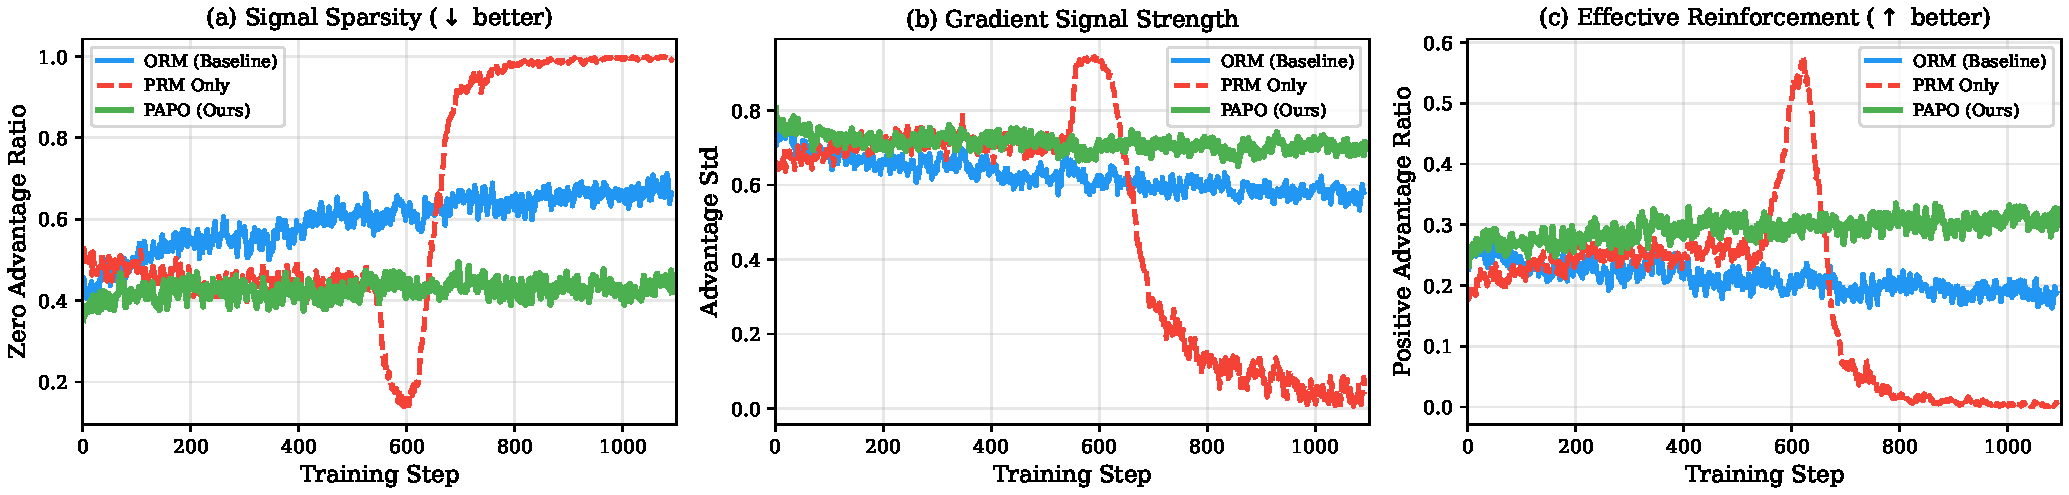
\includegraphics[width=\textwidth]{figures/fig_signal_exhaustion.pdf}
\caption{Signal quality comparison on Qwen2.5-7B. \textbf{(a)} Zero-advantage ratio: ORM's sparsity grows to 69\% while \method{} maintains 44\%. \textbf{(b)} Advantage standard deviation, reflecting gradient signal strength. \textbf{(c)} Positive-advantage ratio, reflecting reinforcement density.}
\label{fig:signal_exhaustion}
\end{figure*}

The widening gap observed in Figure~\ref{fig:hero}a can be traced to signal exhaustion in ORM's advantage computation. We analyze this on Qwen2.5-7B using the metrics in Figure~\ref{fig:signal_exhaustion}.

\paragraph{Signal exhaustion in ORM.} With growing model capability over training, more response groups become uniformly correct and yield zero advantage under ORM. Figure~\ref{fig:signal_exhaustion}a quantifies this trend. The zero-advantage ratio of ORM, defined as the fraction of samples producing zero gradient, rises from approximately 40\% to 69\% over the course of training. By the late training stage, more than two-thirds of samples provide no contribution to learning. The advantage standard deviation in panel b and the positive-advantage ratio in panel c convey a consistent pattern. The gradient signal from ORM gradually becomes sparser and weaker.

\paragraph{Signal preservation in \method{}.} \method{} holds the zero-advantage ratio at ${\sim}44\%$, a 25-point reduction that translates to roughly 80\% more informative samples per batch. This is because $\aproc$ remains active in all-correct groups where $\aout = 0$, differentiating responses by reasoning quality rather than leaving them with zero gradient. The fraction of groups where $\aproc$ activates grows from ${\sim}30\%$ to 70\% as the model improves, providing increasingly dense quality signal precisely as ORM exhausts.

\paragraph{Quality penalization.} Beyond filling zero-signal gaps, $\aproc$ actively discourages sloppy reasoning even among correct responses. The minimum advantage within the correct group reaches $\approx -1.49$ under \method{} compared to identically 0.0 under ORM, meaning correct responses with poor derivations receive negative advantage and are suppressed. This quality pressure is entirely absent in ORM-based GRPO. More detailed analyses of the process advantage effect and advantage composition are provided in Appendix~\ref{sec:rubric-analysis} and~\ref{sec:adv-decomp}.
